% $Id: gui_disres.tex 395 2011-11-17 22:34:59Z cphillip $
%
% Written by J. Schrouff for v2.0
%_______________________________________________


\chapter{Display voxel and region contribution}
\label{chap:DisWeights}
\minitoc

\section{Introduction}

Another important aspect of pattern recognition modelling is to see what the machine has learned - some brain 
areas are probably more informative about class membership/regression targets than others. For example, in a visual
task, we would expect discriminative information in the occipital lobe. This is 
called \textit{information mapping}, and it is of particular import to be critical at this stage - if
the discriminative weight of a machine is concentrated in the eyes, for example, it is important
to correct the analysis mask that was used to exclude them. The question to ask is
``which voxels drive the modelling, and do they make sense with respect to the experimental
paradigm and neurophysiology'' ? In the case of linear kernels, the classifier/regression weight
vector is a linear combination or weighted average of the training examples, and can be plotted
as an image representing a weight map. The \textit{weight map} is therefore a spatial representation
of the decision function, i.e. every voxel contributes with a certain weight to the decision function. 
Pattern recognition models (classifiers or regression functions) are multivariate, i.e. they
take into account correlations in the data. Since the discrimination or prediction is
based on the whole brain pattern, rather than on individual regions or voxels, all voxels
contribute to the classification or regression and no conclusions should be drawn about a particular
subset of voxels in isolation.

Starting from PRoNTo v2.0, it is possible to derive weights at the region level (as anatomically defined by an atlas, from MKL or from summarizing the weights). This window allows to display maps of voxel and of region contribution. Furthermore, the region contributions can be ranked in descending order, yielding a sorted list of regions according to their contribution to the classification/regression model. We hope this will help the interpretation of model parameters in terms of cognitive neuroscience.

\textbf{Important note:} The implemented version of MKL (\cite{Rakotomamonjy2008}) is sparse in the kernel space. This means that only a few regions/modalities will contribute to the model. In the same way, voxel weights derived from MKL models can have perfectly null values, hence not contributing to the model. This therefore eases the interpretation of the weight map, as not all voxels contribute to the decision. However, this selection of regions/modalities might depend on the dataset, and small variations in the dataset (as induced by cross-validation) might lead to different subsets of regions/modalities begin selected. Therefore, care should be taken when reporting selected regions/modalities and each fold should be looked at separately. We also provide a quantification of the variability across folds of the ranking of the regions/modalities (`Expected Ranking') to provide some insights on this issue.


\section{Displaying weights}

To launch the 'Display weights' window, make sure that weight maps have been computed for at least one model (Compute Weights, Chapter~\ref{chap:ComputeWeights}).

In the {\tt Review Options} panel, press {\tt Display weights}. At the ``Select PRT.mat'' window,
navigate to where your {\tt PRT.mat} file is stored (using the left column), and select it in the
right column. The display window then opens (Figure \ref{fig_prt_ui_weights_empty}).

\begin{figure}[h!]
\begin{center}
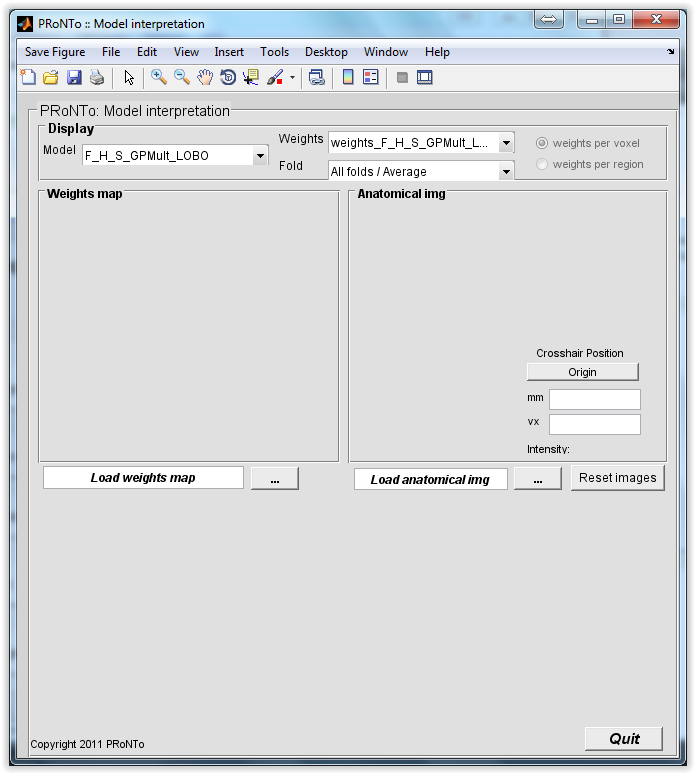
\includegraphics[height=7cm]{images/prt_ui_weights_empty.png}
\caption{Display weights main window after selection of PRT.mat.}
\label{fig_prt_ui_weights_empty}
\end{center}
\end{figure}


The window is divided into four panels; going from top left to bottom left, they
are:
\begin{description}
\item[Display]: this panel allows the user to choose which model and image to display, as well as whether to display the voxel weights or the region contributions.
\item[Weights map]: this displays three projections of the selected weight map and allows to navigate it.
\item[Anatomical img]: if an anatomical image has been loaded, this will display three projections,
and the cross-hair will be synchronised with the weight map.
\item[Additional plots]: this area will display extra information on the model parameters, such as a sorted list of the regions according to their contribution (if weights per region were computed, in the form of a table) and a bar plot of the relative region contribution. If MKL modelling was performed based on multiple modalities, the same table and bar plot will display the relative contributions of each modality to the decision function. 
\end{description}

\subsection{Select image to display}

The \texttt{Display} panel shows the models for which weights were computed and weight images were found in the same folder as the PRT. For each model, the list of images available is displayed in the \texttt{Weights} pop-down list. Typically, one image will be created for a binary comparison or regression with only one modality or multiple modalities concatenated in samples (e.g. multiple runs). On the other hand, multiclass classification models will return one image per class (with the index of the class appended to the name of the image). In the same way, multiple modalities used in multiple kernels will lead to the building of \textit{number of modalities} images. \textbf{Note:} MKL performed on regions of interest as defined by an atlas leads to a whole brain image being created (i.e. a signal image). For each image, the weight map can be displayed for each fold or for their average. In PRoNTo v2.0, it is possible to display the contributions of each voxel (\texttt{weights per voxel}) or of each region (\texttt{weights per region}, if previously computed).

\textbf{Note:} the weight images (per voxel and per region) are automatically detected in the list of files in the PRT folder according to the name specified in the 'Compute weights' step (Chapter \ref{chap:ComputeWeights}). Modifying the image name afterwards or moving the images might lead to warning messages and the images will not be listed in the GUI.

To display a weight image, select a model, an image and a fold. If only weights per voxel were estimated, the window will look similar to Figure \ref{fig_prt_ui_weights_img}.

\begin{figure}[h!]
\begin{center}
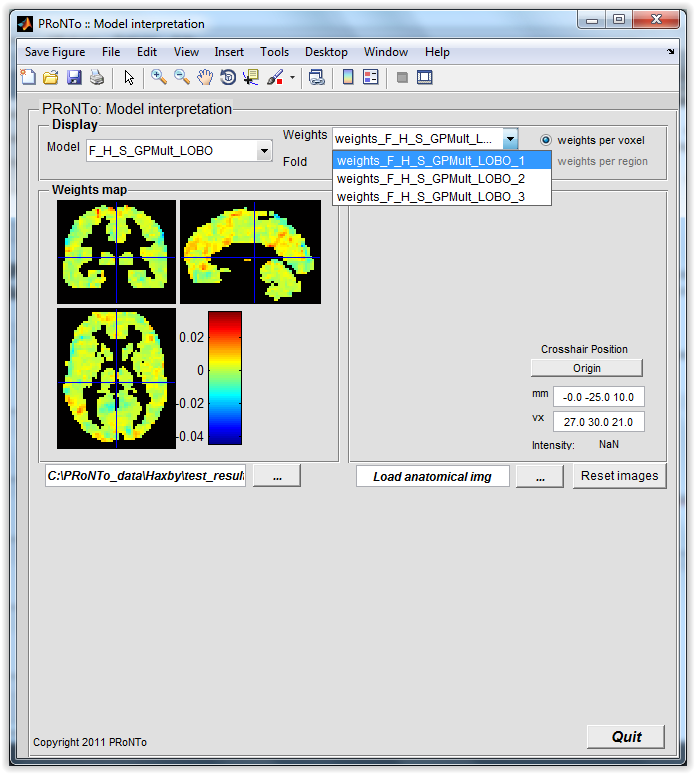
\includegraphics[height=7cm]{images/prt_ui_weights_img.png}
\caption{Displaying weight image for class 1 of a three-class GP model (Haxby dataset).}
\label{fig_prt_ui_weights_img}
\end{center}
\end{figure}

\subsection{Weights map}

The weight map is displayed with a cross-hair and a colorbar. The colorbar indicates the
relative importance of the voxel in the decision function of the machine. This value is also
indicated in the {\tt intensity} field of the {\tt Anatomical img} panel. Note that all voxels
in the mask contribute to the decision function, since the analysis is multivariate. Contrary
to common practice in Statistical Parametric Mapping, which is a mass-univariate approach, {\em it does
not make sense to isolate part of the pattern and report only on the peaks of the distribution
of the decision function's weight map}. 


\subsection{Anatomical image}
By clicking on the $[${\tt ...}$]$ button next to the {\tt Load weight map} field, 
a dialogue opens that allows you to select the weight map {\tt .img} file that 
was computed previously (see Chapter~\ref{chap:ComputeWeights} for the procedure).
Similarly, a co-registered anatomical image can be loaded in the {\tt Anatomical img}
pane of the window. See Figure~\ref{fig_prt_ui_results_WM_anatomical} for an example.

\subsection{Additional plots}

\subsubsection{Sorted table of region/modality contributions}

\subsubsection{Bar plot of contributions}





